\documentclass[8pt,a4paper,compress]{beamer}

\usepackage{/home/siyer/lib/slides}

\title{String Sorts}
\date{}
\begin{document}
\begin{frame}
\vfill
\titlepage
\end{frame}

\begin{frame}
\frametitle{Outline}
\tableofcontents
\end{frame}

\section{Rules of the Game}
\begin{frame}[fragile]
\pause

Our implementations of string algorithms are expressed in terms of the Java \lstinline{String} class

\pause
\bigskip

Important characteristics of Java strings
\begin{itemize}
\item A \lstinline{String} is a sequence of characters, each of type \lstinline{char} and having one of $2^{16}$ possible values
\item \lstinline{String} objects are immutable
\item The \lstinline{charAt()} method that extracts a specified character from a string operates in constant time
\item The \lstinline{length()} method that returns the length of a string operates in constant time
\item The \lstinline{substring()} method that extracts a specified substring operates in constant time
\item Appending one string to another using the \lstinline{+} operator takes time proportional to the length of the result
\item \lstinline{String} is not a primitive type, but wraps a low-level representation, which is as an array of \lstinline{char} values
\end{itemize}

\pause
\bigskip

Our implementations make liberal use of indexing and length and occasional use of substring extraction and concatenation

\pause
\bigskip

We will use $R$ (for radix) to denote the number of characters in an alphabet

\pause
\bigskip

Our alphabet will be the extended ASCII character set, with $R=256$
\end{frame}

\section{Key-indexed Counting}
\begin{frame}[fragile]
\pause

Key-indexed counting is a simple method for sorting that is effective whenever the keys are small integers, as in the following example

\begin{center}
\visible<2->{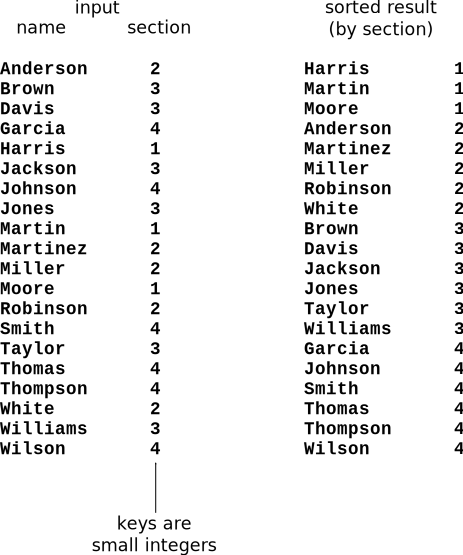
\includegraphics[scale=0.35]{figures/kic1.pdf}}
\end{center}

\pause
\bigskip

The sorting method involves four steps
\end{frame}

\begin{frame}[fragile]
\pause

Compute frequency counts: the first step is to count the frequency of occurrence of each key value, using an \lstinline{int} array \lstinline{count[]}

\begin{lstlisting}[language=Java]
for (i = 0; i < N; i++) {
    count[a[i].key() + 1]++;
}
\end{lstlisting}

\begin{center}
\visible<2->{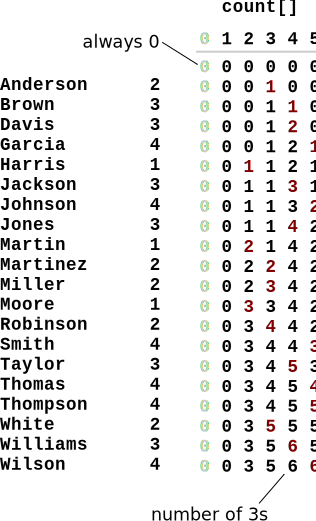
\includegraphics[scale=0.35]{figures/kic2.pdf}}
\end{center}
\end{frame}

\begin{frame}[fragile]
\pause

Transform counts to indices: the second step is to use \lstinline{count[]} to compute, for each key value, the starting index positions in the sorted order of items with that key

\begin{lstlisting}[language=Java]
for (int r = 0; r < R; r++) {
    count[r + 1] += count[r];
}
\end{lstlisting}

\begin{center}
\visible<2->{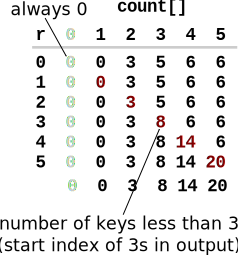
\includegraphics[scale=0.4]{figures/kic3.pdf}}
\end{center}
\end{frame}

\begin{frame}[fragile]
\pause

Distribute the data: the third step is to use the index table \lstinline{count[]} to move the items to an auxiliary array \lstinline{aux[]}

\begin{lstlisting}[language=Java]
for (int i = 0; i < N; i++) {
    aux[count[a[i].key()]++] = a[i];
}
\end{lstlisting}

\begin{center}
\visible<2->{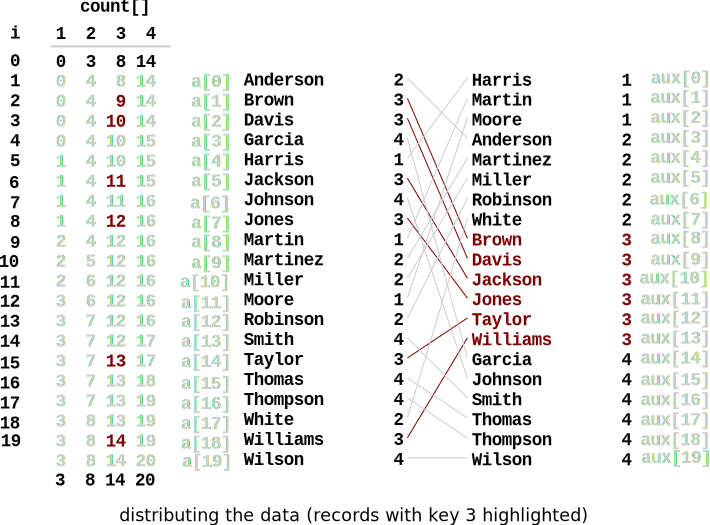
\includegraphics[scale=0.35]{figures/kic4.pdf}}
\end{center}

\pause
\bigskip

Copy back: the last step is to copy the sorted result back to the original array

\begin{lstlisting}[language=Java]
for (int i = 0; i < N; i++) {
    a[i] = aux[i];
}
\end{lstlisting}
\end{frame}

\begin{frame}[fragile]
\pause

Key-indexed counting (\lstinline{a[i].key} is an integer in $[0, R-1]$)
\begin{lstlisting}[language=Java]
int N = a.length;
String[] aux = new String[N];
int[] count = new int[R + 1];

// Compute frequency counts.
for (int i = 0; i < N; i++) { 
    count[a[i].key() + 1]++;
}

// Transform counts to indices.
for (int r = 0; r < R; r++) {
    count[r+1] += count[r];
}

// Distribute the records.
for (int i = 0; i < N; i++) {
    aux[count[a[i].key()]++] = a[i];
}

// Copy back.
for (int i = 0; i < N; i++) {
    a[i] = aux[i];
}
\end{lstlisting}

\pause
\bigskip

Key-indexed counting uses $8N + 3R + 1$ array accesses to stably
sort $N$ items whose keys are integers between 0 and $R - 1$
\end{frame}

\section{LSD String Sort}
\begin{frame}[fragile]
\pause

Least-significant-digit first (LSD) string sort is a sorting method for fixed-length strings, as in the following example

\begin{center}
\visible<2->{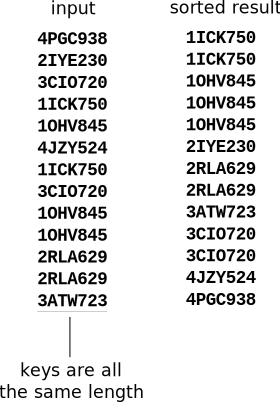
\includegraphics[scale=0.45]{figures/lsd1.pdf}}
\end{center}

\pause
\bigskip

Such strings can be sorted using key-indexed counting

\pause
\bigskip

If the strings are each of length $W$, we sort the strings $W$ times with key-indexed counting, using each of the positions as the key, proceeding from right to left
\end{frame}

\begin{frame}[fragile]
\pause

\begin{lstlisting}[language=Java]
package edu.princeton.cs.algs4;

public class LSD {
    private static final int R = 256; 

    public static void sort(String[] a, int W) {
        int N = a.length;
        String[] aux = new String[N];
        for (int d = W - 1; d >= 0; d--) {
            int[] count = new int[R+1];
            for (int i = 0; i < N; i++) { count[a[i].charAt(d) + 1]++; }
            for (int r = 0; r < R; r++) { count[r+1] += count[r]; }
            for (int i = 0; i < N; i++) { aux[count[a[i].charAt(d)]++] = a[i]; }
            for (int i = 0; i < N; i++) { a[i] = aux[i]; }
        }
    }

    public static void main(String[] args) {
        String[] a = StdIn.readAllStrings();
        int N = a.length;
        int W = a[0].length();
        for (int i = 0; i < N; i++) {
            assert a[i].length() == W : "Strings must have fixed length";
        }
        sort(a, W);
        for (int i = 0; i < N; i++) }
            StdOut.println(a[i]);
        }
    }
}
\end{lstlisting}
\end{frame}

\begin{frame}[fragile]
\pause

\begin{lstlisting}[language={}]
$ more words3.txt
bed bug dad yes zoo
now for tip ilk dim 
tag jot sob nob sky
hut men egg few jay
owl joy rap gig wee
was wad fee tap tar
dug jam all bad yet
\end{lstlisting}

\pause

\begin{lstlisting}[language={}]
$ java edu.princeton.cs.algs4.LSD < words3.txt 
all
bad
bed
bug
dad
...
yes
yet
zoo
\end{lstlisting}
\end{frame}

\begin{frame}[fragile]
\pause

Trace

\begin{center}
\visible<2->{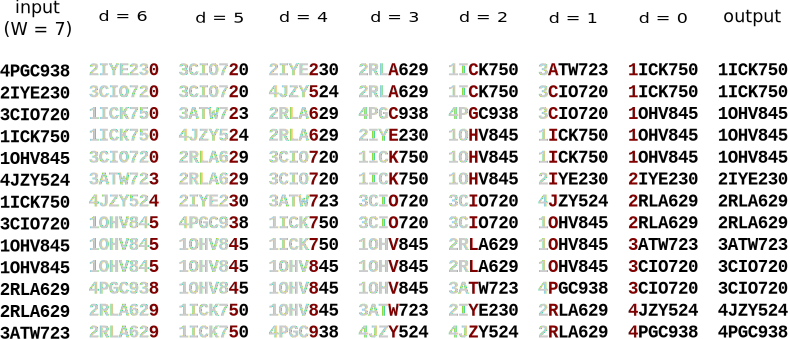
\includegraphics[scale=0.45]{figures/lsd2.pdf}}
\end{center}

\pause
\bigskip

LSD string sort uses $\sim 7WN + 3WR$ array accesses and
extra space proportional to $N + R$ to sort $N$ items whose keys are $W$-character strings taken from an $R$-character alphabet
\end{frame}

\section{MSD String Sort}
\begin{frame}[fragile]
\pause

Most-significant-digit first (MSD) string sort is a general-purpose string sort, where strings are not necessarily all the same length, as in the following example

\begin{center}
\visible<2->{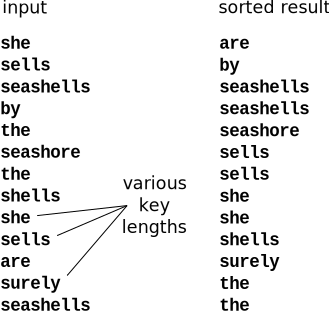
\includegraphics[scale=0.4]{figures/msd1.pdf}}
\end{center}

\pause
\bigskip

The method uses key-indexed counting to sort the strings according to
their first character, then (recursively) sorts the subarrays corresponding to each character
\end{frame}

\begin{frame}[fragile]
\pause

We use a private two-argument \lstinline{charAt()} method to convert from an indexed string character to an array index that returns -1 if the specified character position is past the end of the string

\pause
\bigskip

We add 1 to each returned value of \lstinline{charAt()}, to get a nonnegative integer that we can use to index \lstinline{count[]}

\pause
\bigskip

The above convention means that we have $R+1$ different possible character values at each string position: 0 to signify end of string,
1 for the first alphabet character, 2 for the second alphabet
character, and so forth
\end{frame}

\begin{frame}[fragile]
\pause

\begin{lstlisting}[language=Java]
package edu.princeton.cs.algs4;

public class MSD {
    private static final int R      = 256; 
    private static final int CUTOFF =  15; 
    
    private static int charAt(String s, int d) {
        return (d == s.length()) ? -1 : s.charAt(d);
    }

    public static void sort(String[] a) {
        int N = a.length;
        String[] aux = new String[N];
        sort(a, 0, N - 1, 0, aux);
    }

    private static void sort(String[] a, int lo, int hi, int d, String[] aux) {
        if (hi <= lo + CUTOFF) { insertion(a, lo, hi, d); return; }
        int[] count = new int[R + 2];
        for (int i = lo; i <= hi; i++) {
            int c = charAt(a[i], d);
            count[c + 2]++;
        }
        for (int r = 0; r < R + 1; r++) { count[r + 1] += count[r]; }
        for (int i = lo; i <= hi; i++) {
            int c = charAt(a[i], d);
            aux[count[c + 1]++] = a[i];
        }
        for (int i = lo; i <= hi; i++) { a[i] = aux[i - lo]; }
        for (int r = 0; r < R; r++) {
            sort(a, lo + count[r], lo + count[r + 1] - 1, d + 1, aux);
        }
    }
\end{lstlisting}
\end{frame}

\begin{frame}[fragile]
\pause

\begin{lstlisting}[language=Java]
    private static void insertion(String[] a, int lo, int hi, int d) {
        for (int i = lo; i <= hi; i++) {
            for (int j = i; j > lo && less(a[j], a[j - 1], d); j--) {
                exch(a, j, j - 1);
            }
        }
    }

    private static void exch(String[] a, int i, int j) {
        String temp = a[i];
        a[i] = a[j];
        a[j] = temp;
    }

    private static boolean less(String v, String w, int d) {
        for (int i = d; i < Math.min(v.length(), w.length()); i++) {
            if (v.charAt(i) < w.charAt(i)) { return true; }
            if (v.charAt(i) > w.charAt(i)) { return false; }
        }
        return v.length() < w.length();
    }

    public static void sort(int[] a) {
        int N = a.length;
        int[] aux = new int[N];
        sort(a, 0, N - 1, 0, aux);
    }

    public static void main(String[] args) {
        String[] a = StdIn.readAllStrings();
        int N = a.length;
        sort(a);
        for (int i = 0; i < N; i++) { StdOut.println(a[i]); }
    }
}
\end{lstlisting}
\end{frame}

\begin{frame}[fragile]
\pause

\begin{lstlisting}[language={}]
$ more shells.txt 
she sells seashells by the sea shore
the shells she sells are surely seashells
\end{lstlisting}

\pause

\begin{lstlisting}[language={}]
$ java edu.princeton.cs.algs4.MSD < shells.txt 
txt 
are
by
sea
seashells
seashells
sells
sells
she
she
shells
shore
surely
the
the
\end{lstlisting}
\end{frame}

\begin{frame}[fragile]
\pause

Trace: top level of \lstinline{sort(a, 0, 14, 0)}

\begin{center}
\visible<2->{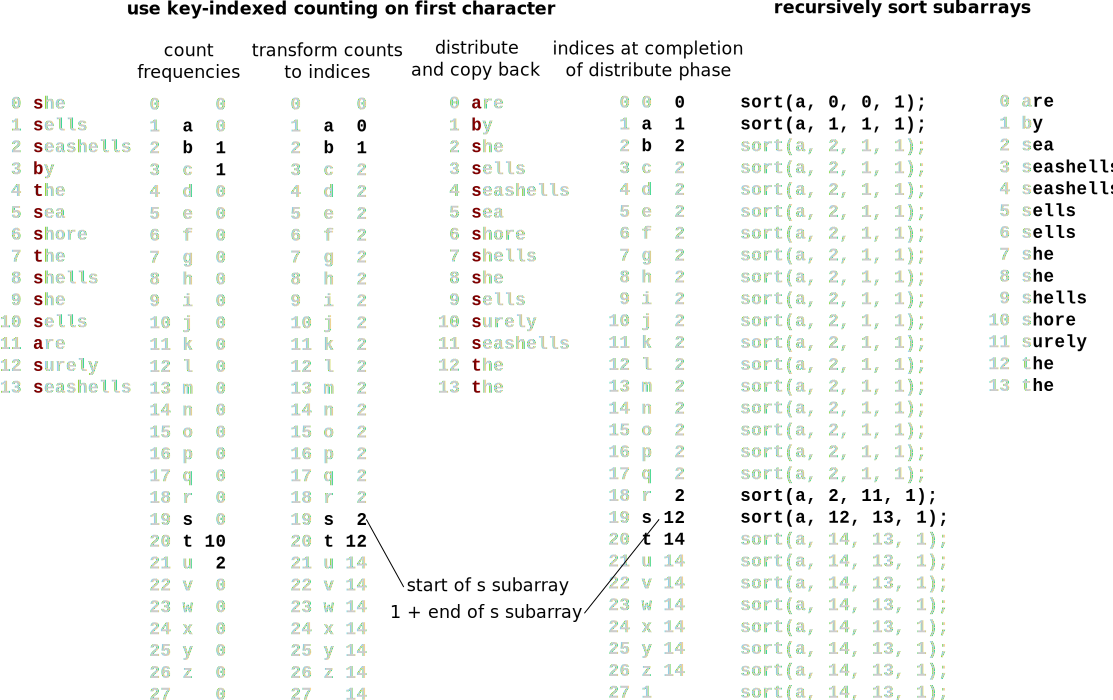
\includegraphics[scale=0.3]{figures/msd2.pdf}}
\end{center}

To sort $N$ random strings from an $R$-character alphabet, MSD string sort examines about $N \log_R N$ characters, on average

\pause
\bigskip

MSD string sort uses between $8N + 3R$ and $\sim 7wN + 3WR$ array accesses
to sort $N$ strings taken from an $R$-character alphabet, where $w$ is the average string length
\end{frame}

\section{Performance Characteristics of String-sorting Algorithms}
\begin{frame}[fragile]
\pause

\begin{center}
\begin{tabular}{cccccc}
algorithm & stable? & inplace? & running time$^\dagger$ & extra space$^\ddagger$ & sweet spot \\ \hline

\makecell{insertion sort \\ for strings} & yes & yes & \makecell{between \\ $N$ and $N^2$} & 1 & \makecell{small arrays, \\ arrays in order} \\

quick sort & no & yes & $N \log^2 N$ & $\log N$ & \makecell{general purpose \\ when space \\ is tight} \\

merge sort & yes & no & $N \log^2 N$ & $N$ & \makecell{general purpose \\ stable sort} \\

\makecell{3-way quick \\ sort} & no & yes & \makecell{between \\ $N$ and $N\log N$} & $\log N$ & \makecell{large numbers \\ of equal keys} \\

\makecell{LSD string \\ sort} & yes & no & $NW$ & $N$ & \makecell{short fixed \\ length strings} \\

\makecell{MSD string \\ sort} & yes & no & \makecell{between \\ $N$ and $Nw$} & $N + WR$ & random strings \\

\makecell{3-way string \\ quick sort} & no & yes & \makecell{between \\ $N$ and $Nw$} & $W + \log N$ & \makecell{general purpose \\ strings with \\ long prefix \\ matches}
\end{tabular} 

\bigskip

$\dagger \ddagger$ Order of growth of typical number of calls to \lstinline{charAt()} to sort $N$ strings from an $R$-character alphabet (average length $w$, max length $W$)
\end{center}
\end{frame}

\end{document}
